\chapter{Presentation of results}
\label{cha:results}
\section{Influence of $B_{cr}$ and its origin}
\label{sec:reactivity}

\subsection{Impact on the effective multiplication factor}
In order to have a basic idea of how much the burnup of control rods
could effect the fuel assembly, we compare the effective multiplication factor.

Using the model described in section \ref{sec:model},
we calculate two sets of fuel assemblies.
One has their control rods set as a burnable material,
the other set as a non-burnable material.
The effective multiplication factor in these two conditions is shown in Fig \ref{fig:k_bu}.
\begin{figure}[!htb]
    \centering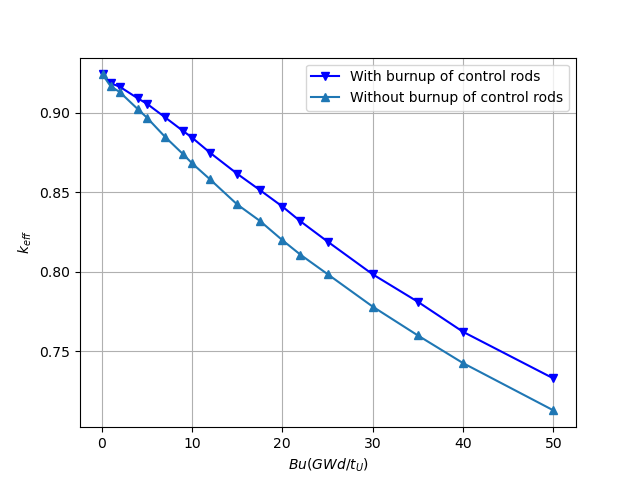
\includegraphics[width=0.5\linewidth]{Figs/keff_bu_dififBcr.png}
    \caption{Effective multiplication factor as a function of fuel assembly burnup}
    \label{fig:k_bu}
\end{figure}

The results show that, after a burnup of \textit{20 GWd/tU},
the difference in $k_{eff}$ could reach \textit{2000 ppm}.
It is a gap that could not be neglected.
This confirms that in these kinds of nuclear reactors, where control rods are inserted in
long periods of time, the burnup of control rods is a factor that mush be considered.


\subsection{Origin of $B_{cr}$}
\label{sec:material}
In order to track the origin of this phenomena,
the atom density of different nuclides in control rods is recorded.
Fig \ref{fig:nuclide_change} shows the change of atom density of different
nuclides as a function of the burnup of fuel.

\begin{figure}[!htb]
    \centering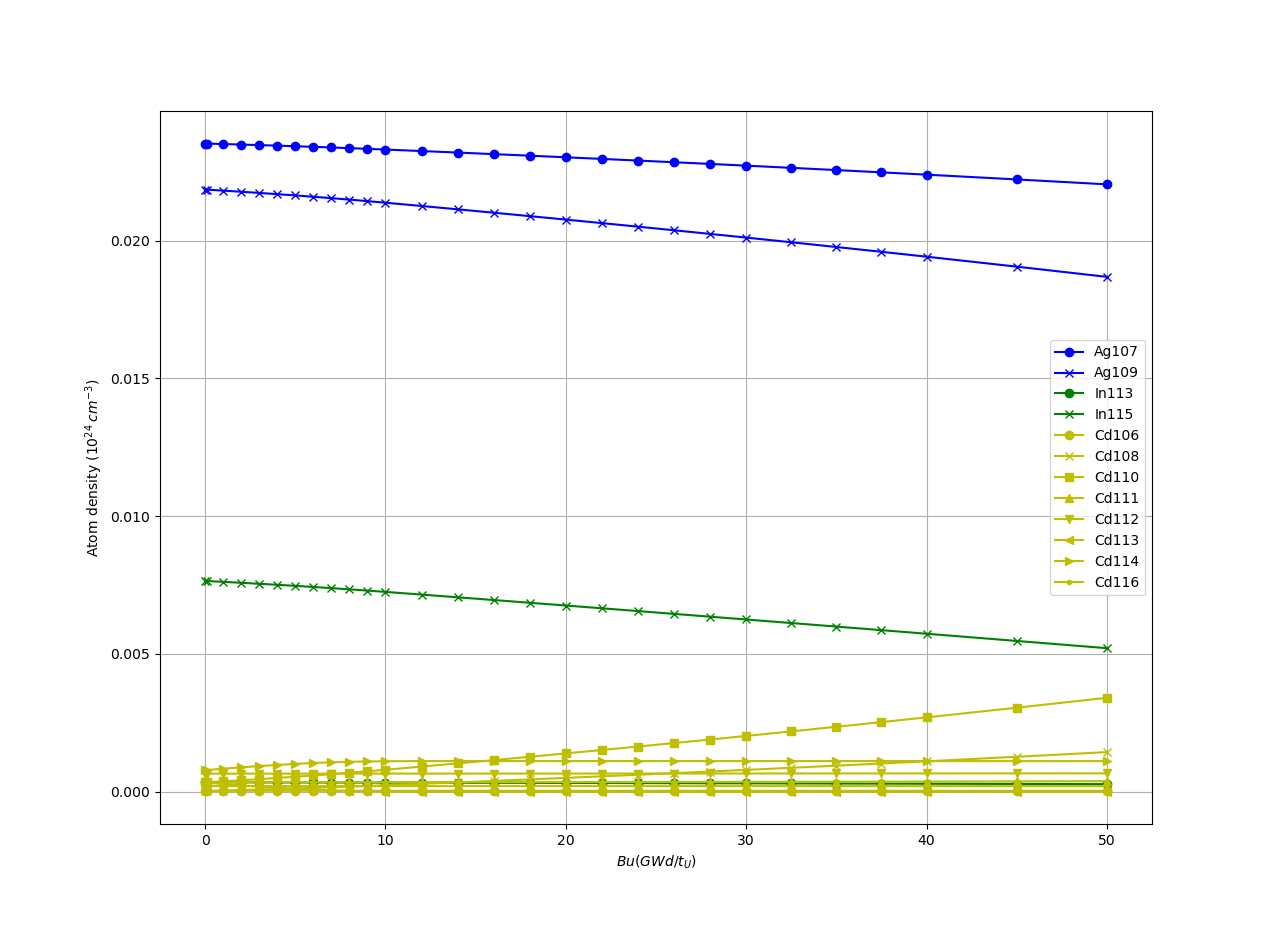
\includegraphics[width=0.7\linewidth]{Figs/Ni_Bu.png}
    \caption{Nuclide atom density change as a function of fuel burnup}
    \label{fig:nuclide_change}
\end{figure}

\textit{Ag107}($\sigma_h = \textit{45.2 barn}$), \textit{Ag109}($\sigma_h = \textit{92.8 barn}$)
and \textit{In115}($\sigma_h = \textit{203.7 barn}$) are the three main hot neutron absorber nuclides in control rods.
Their atom density decreases very fast compared to other nuclides.
After absorbing a neutron, they transfer to nuclides of other elements (mainly \textit{Cd} and \textit{Sn})
whose hot neutron absorption cross section is much smaller.
This reduces the macroscopic hot neutron absorption cross section of control rods
and causes the burnup of control rods.

\section{Quantification of the burnup of control rods}
\label{sec:quantification_results}
Introducing the quantification method described in section \ref{sec:quantification_methods} as the new representation of the burnup of control rods,
we could get figure \ref{fig:bcr0-bcr}.
$k$ is calculated to be \textit{0.03} using only the three main neutron absorbing nuclide \textit{Ag107}, \textit{Ag109}
and \textit{In115}.

\begin{figure}[!htb]
    \centering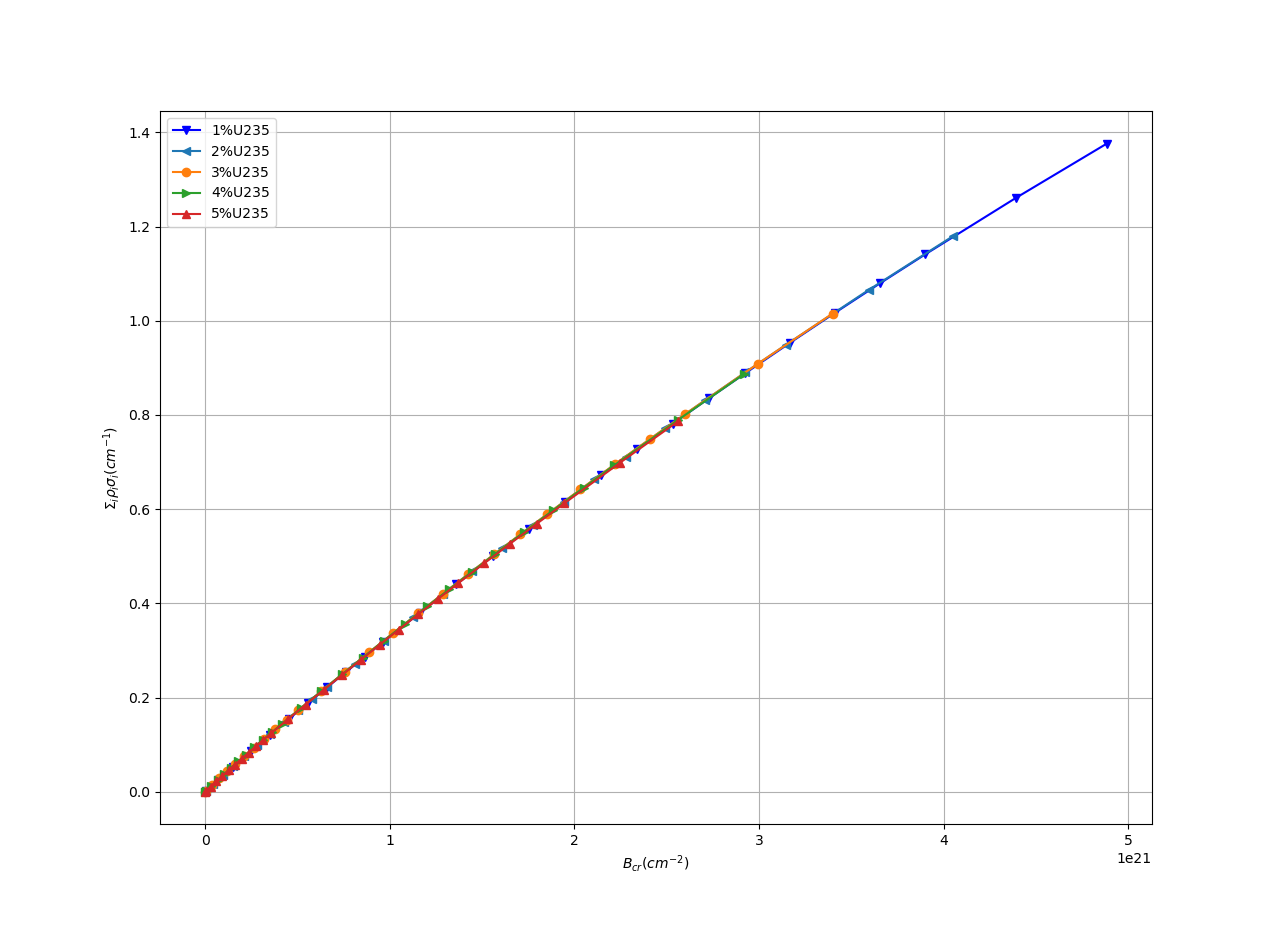
\includegraphics[width=0.6\linewidth]{Figs/Bcr0_Bcro_difU.png}
    \caption{$B_{cr0}$ as a function of $B_{cr}$ using control rod's neutron fluxes for different enrichments}
    \label{fig:bcr0-bcr}
\end{figure}

However, in some simulation softwares, it is still quite difficult to access to the neutron flux density in control rods.
Simulation results show that it can be replaced by the average neutron flux density in the fuel assembly with a different $k$
(\textit{0.1} in our case).
For the model we built, differences in \textit{U235} enrichment, moderator density,
moderator temperature and boron concentration are tested
to have no effect on $k$. As shown in Figure \ref{fig:k_differences}.

\begin{figure}[!htb]
    \centering
    \begin{subfigure}[b]{.475\textwidth}
        \centering
        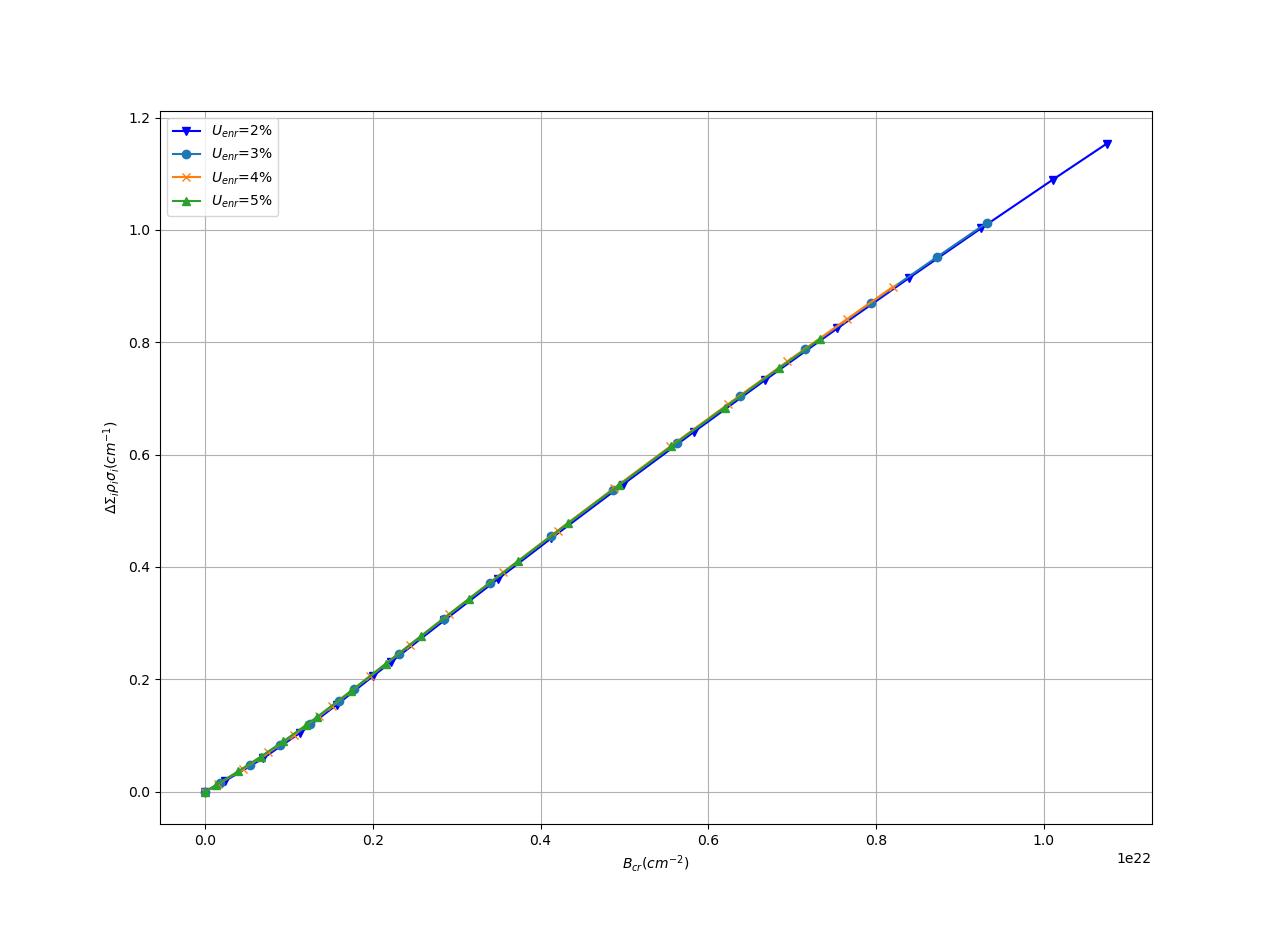
\includegraphics[width=\textwidth]{Figs/Bcr0_Bcr_difU.png}
        \caption{Different enrichment}
        \label{fig:diffU}
    \end{subfigure}%
    \hfill
    \begin{subfigure}[b]{.475\textwidth}
        \centering
        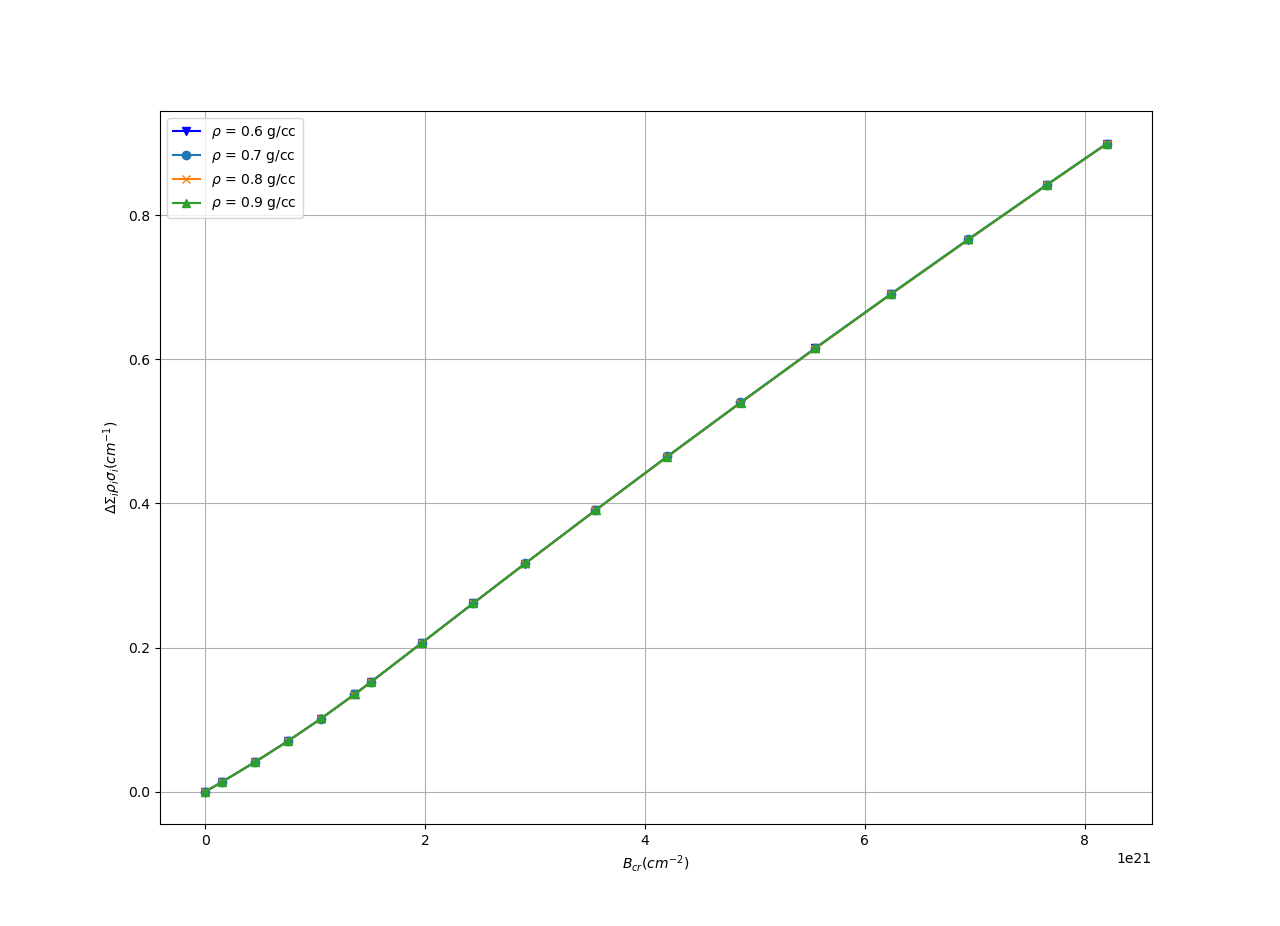
\includegraphics[width=\textwidth]{Figs/Bcr0_Bcr_difwd.png}
        \caption{Different moderator density}
        \label{fig:diffwd}
    \end{subfigure}
    \vskip\baselineskip
    \begin{subfigure}[b]{.475\textwidth}
        \centering
        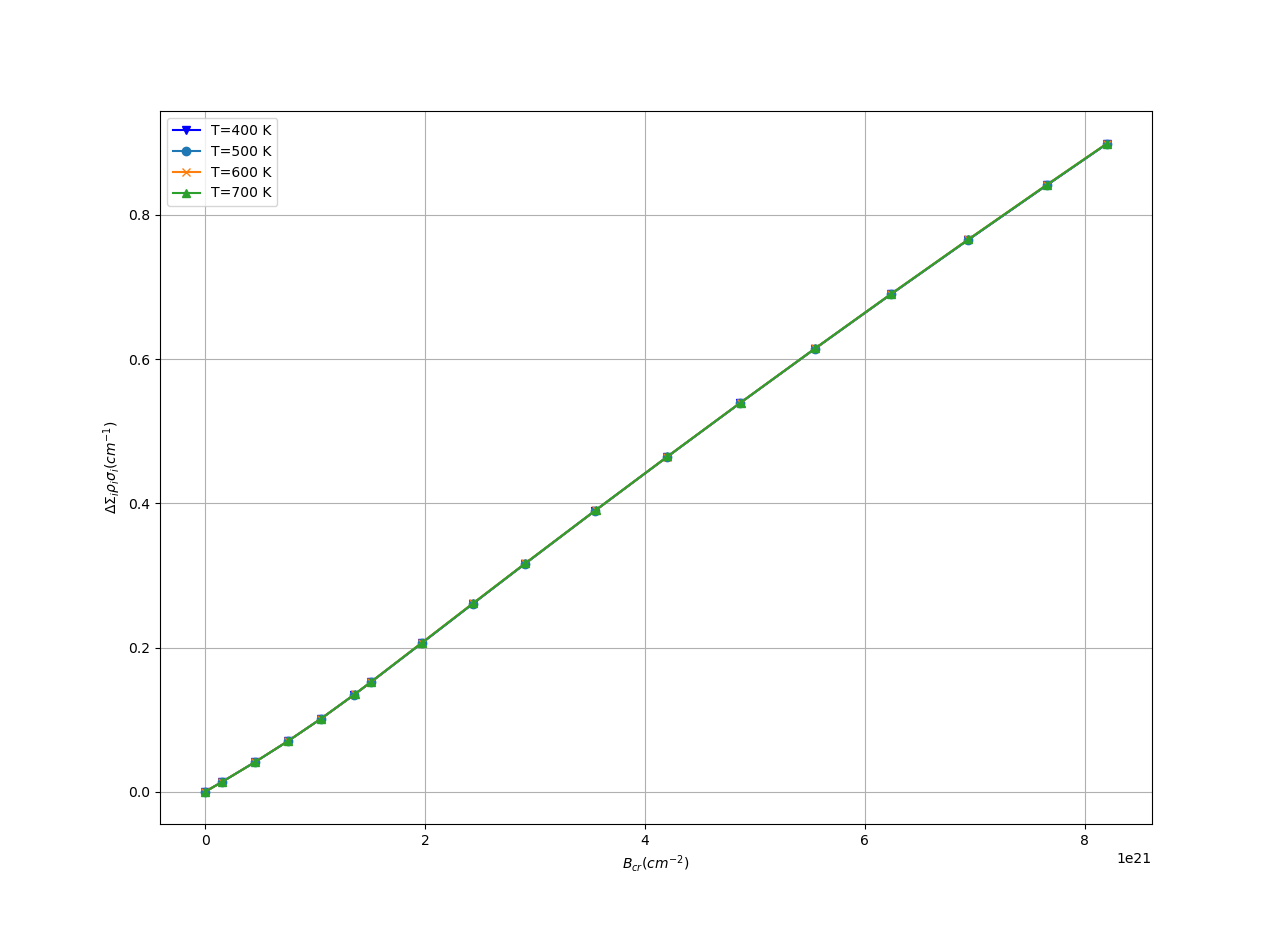
\includegraphics[width=\textwidth]{Figs/Bcr0_Bcr_difT.png}
        \caption{Different temperature}
        \label{fig:diffT}
    \end{subfigure}%
    \hfill
    \begin{subfigure}[b]{.475\textwidth}
        \centering
        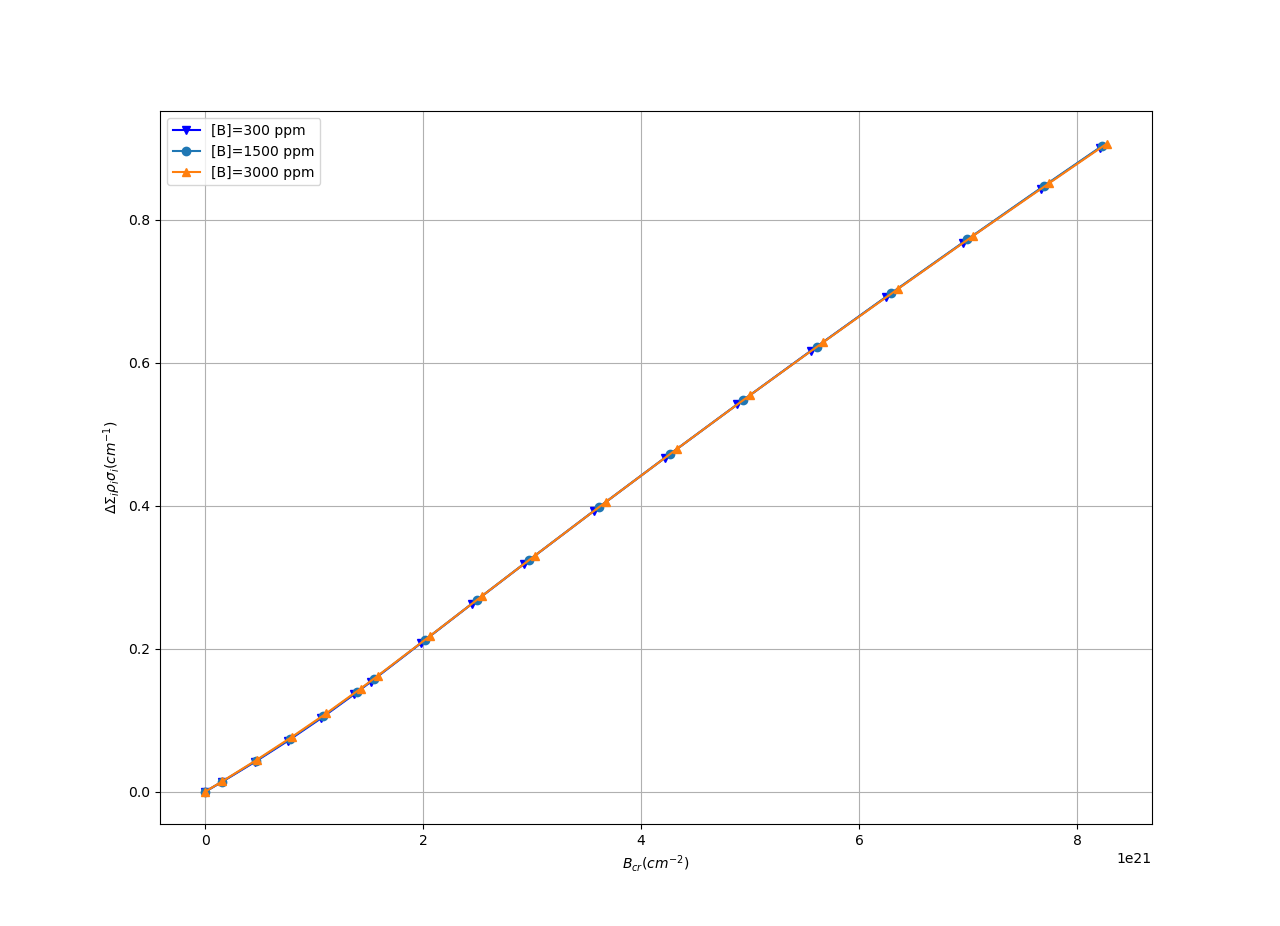
\includegraphics[width=\textwidth]{Figs/Bcr0_Bcr_difB.png}
        \caption{Different boron concentration}
        \label{fig:diffB}
    \end{subfigure}
    \caption{$B_{cr0}$ as a function of $B_{cr}$ using assembly's average neutron fluxes in different conditions}
    \label{fig:k_differences}
\end{figure}

In the following sections, we'll use $B_{cr}$ calculated with average neutron flux density
in fuel assembly to quantify the burnup of control rods.

\section{Results of the Deep Neuron Network}
\label{sec:dnn}

\subsection{Regress results}
\label{sec:regression_results}

\textit{N = 550} couples of $(\Delta \Sigma^{cr}, C_B, T, \rho, B_{cr})_n$ were calculated using the
methods introduced in section \ref{sec:neuron_network_setup}.
Several trainings are performed to avoid random effect.
It takes averagely 1500 steps to train the model with \textit{550} data points.
The training process is fairly fast.
The mean absolute error of the model on test data set is around \textit{5} which means a mean relative error smaller
than \textit{1\%}.
The predictions of the test set comparing to the true values are shown in Fig \ref{fig:result1}.

\begin{figure}[!htb]
    \centering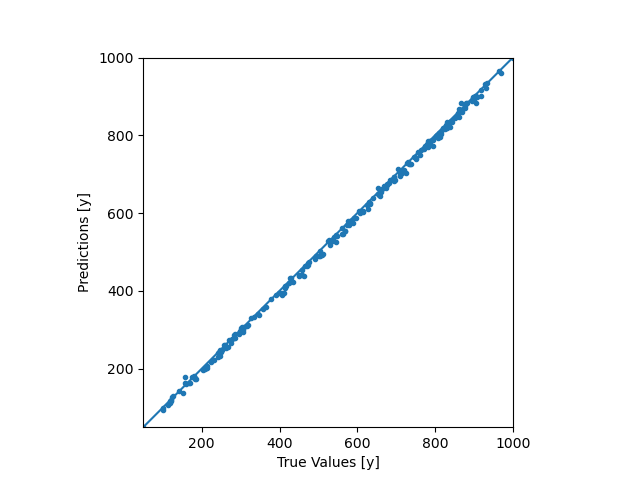
\includegraphics[width=0.6\linewidth]{Figs/DNN_result.png}
    \caption{Deep neuron network predictions comparing to true values}
    \label{fig:result1}
\end{figure}

Considering the errors introduced by the Monte Carlo simulation software itself, the result is very well fitted.
The precision is also good enough for further usage in reactor core simulation softwares.


\section{Discussion}
\label{sec:discussion}

Without any manipulations, it could be found from original data points
that $B_{cr}$'s effect on $\Delta\Sigma^{cr}$ is much greater than others'.
As shown in Figure \ref{fig:datapoints}.
There is an apparent relation between $\Delta\Sigma^{cr}$ and $B_{cr}$ while
other parameters introduce small changes based on this relation.
\begin{figure}[!htb]
    \centering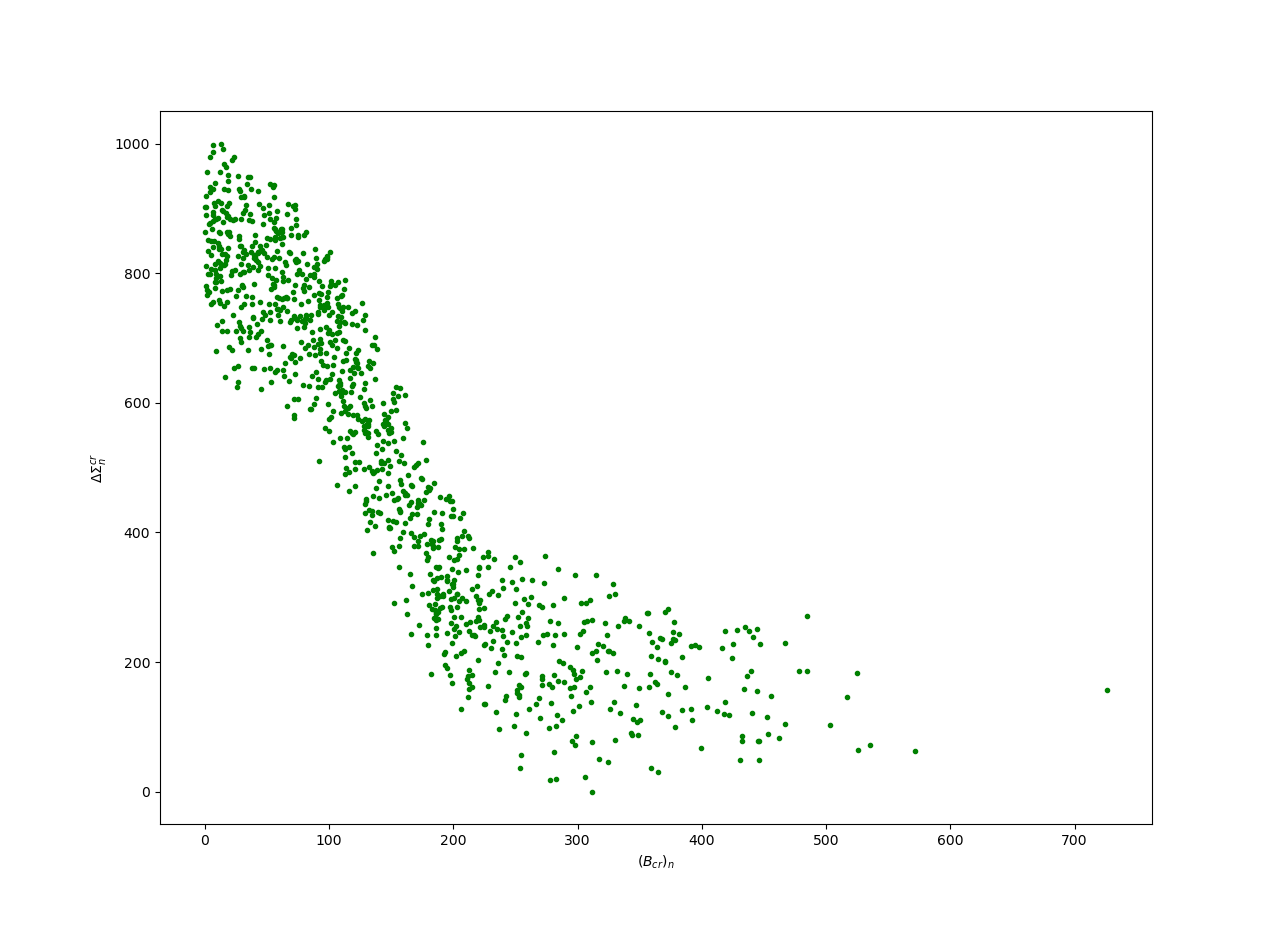
\includegraphics[width=0.5\linewidth]{Figs/data.png}
    \caption{Data points}
    \label{fig:datapoints}
\end{figure}

To study how much $C_B$ or $\rho$ could effect $\Delta\Sigma^{cr}$,
we use the model trained to draw $\Delta\Sigma^{cr}$ as a function of $B_{cr}$ in different conditions
(These are lines that take $B_{cr}$ as x axis with specific $C_B,\:\rho$ values.).
As shown in Fig \ref{fig:Bwdmaxmin}.
\begin{figure}[!htb]
    \centering
    \begin{subfigure}[b]{.475\textwidth}
        \centering
        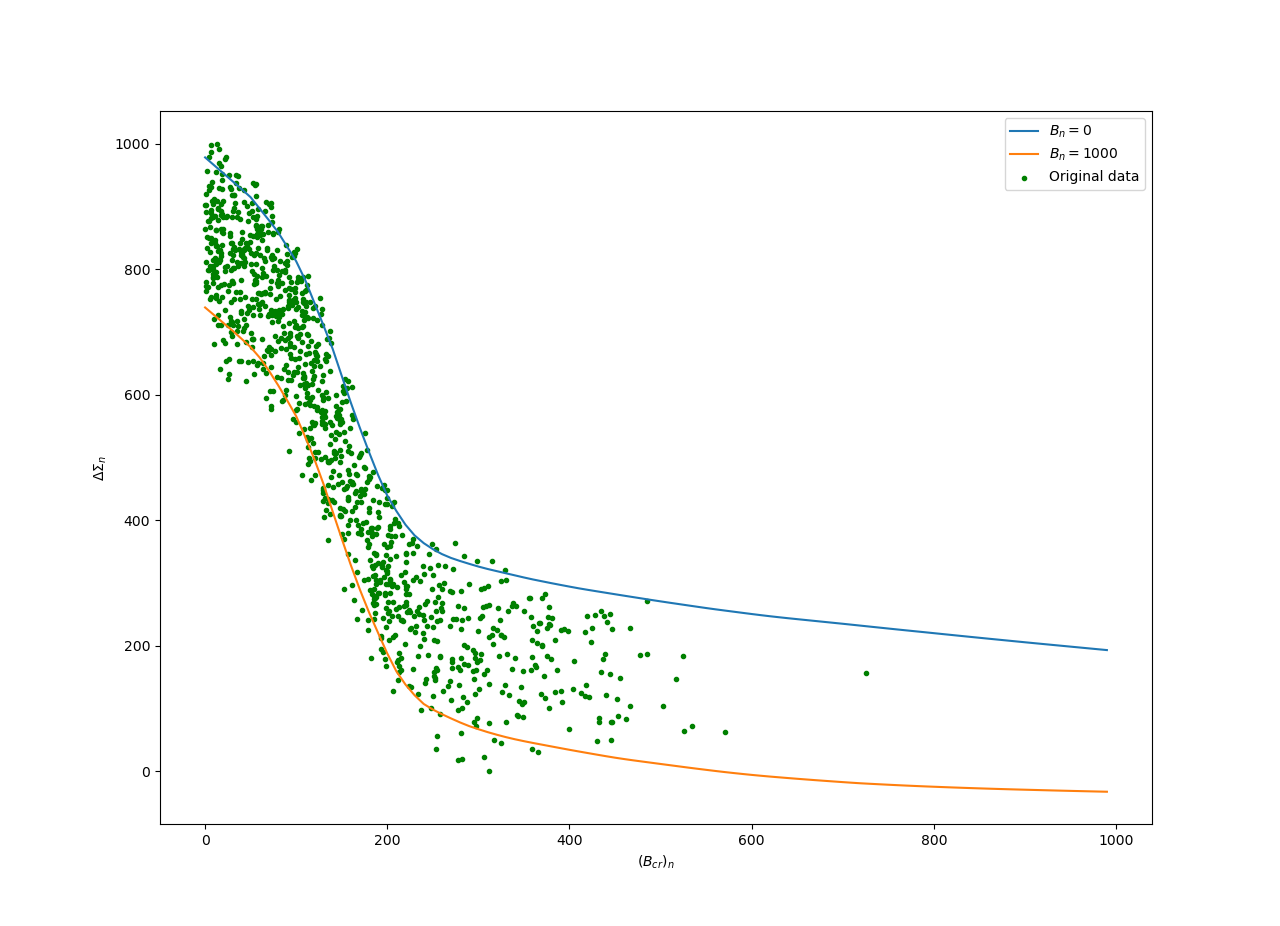
\includegraphics[width=\textwidth]{Figs/DBcr0n_Bcr_difB_DNN.png}
        \caption{Boron concentration's effect}
        \label{fig:EdiffB}
    \end{subfigure}%
    \hfill
    \begin{subfigure}[b]{.475\textwidth}
        \centering
        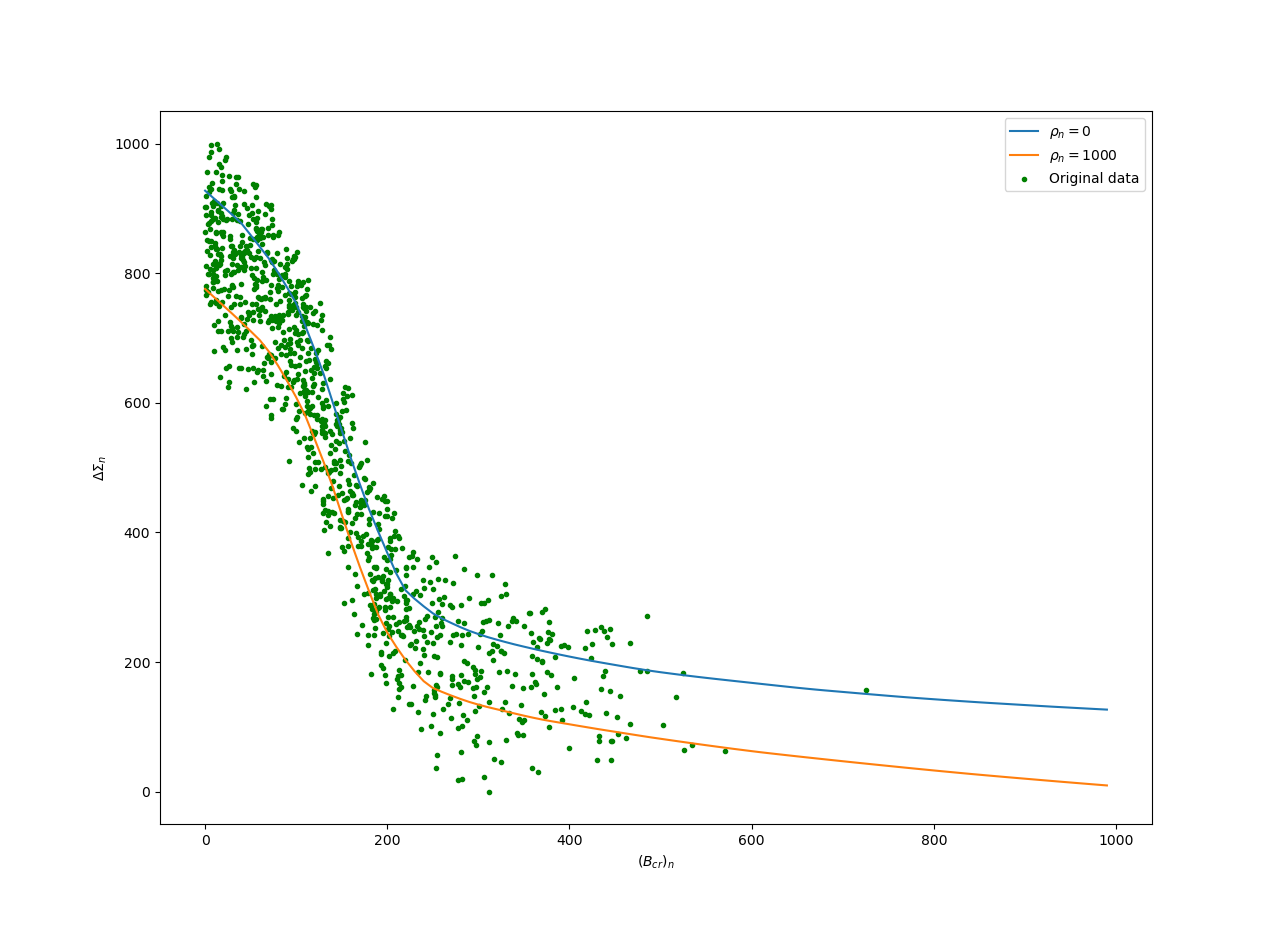
\includegraphics[width=\textwidth]{Figs/DBcr0n_Bcr_difwd_DNN.png}
        \caption{Moderator density's effect}
        \label{fig:Ediffwd}
    \end{subfigure}
    \caption{$\Delta\Sigma^{cr}$ as a function of $B_{cr}$, solid lines are predictions of the model}
    \label{fig:Bwdmaxmin}
\end{figure}

These figures show that no matter the value of $C_B$ or $\rho$, $\Delta\Sigma^{cr}$ drop with the same
tendency as $B_{cr}$ increases.
The correlation between the effect of burnup of control rods and born concentration or water density is not clear.
Note that this is not the relation between $\Delta\Sigma^{cr}$ and $C_B$ or $\rho$ but the
relation between $F$ (defined in section \ref{sec:purpose} in equation \ref{eq:burnup_correction_factor} and \ref{eq:DeltaSigmaF})
and $C_B$ or $\rho$.
The effect of the \textbf{burnup} of control rods is also related to $C_B$ and $\rho$.
If we calculate the burnup correction factor $F$
we could see that the effect of burnup of control rods is indeed related to $C_B$ and $\rho$,
as shown in figure \ref{fig:Fdif},
especially for born concentration at high burnup of control rods.
\begin{figure}[!htb]
    \centering
    \begin{subfigure}[b]{.475\textwidth}
        \centering
        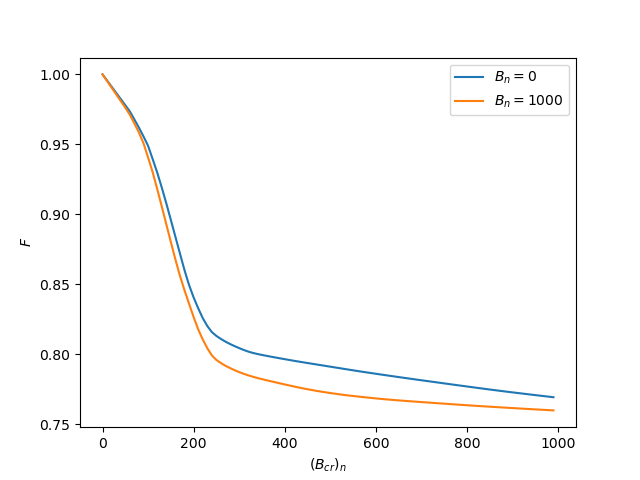
\includegraphics[width=\textwidth]{Figs/F_Bcr_difB.png}
        \caption{Boron concentration's effect}
        \label{fig:FdiffB}
    \end{subfigure}%
    \hfill
    \begin{subfigure}[b]{.475\textwidth}
        \centering
        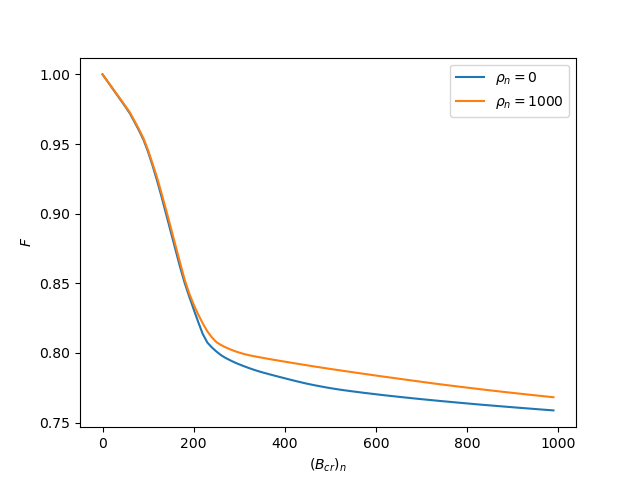
\includegraphics[width=\textwidth]{Figs/F_Bcr_difwd.png}
        \caption{Moderator density's effect}
        \label{fig:Fdiffwd}
    \end{subfigure}
    \caption{$F$ as a function of $B_{cr}$}
    \label{fig:Fdif}
\end{figure}



\chapter{Conclusion}
A relatively ease-to-access quantification of the burnup of control rods is proposed with verifications done in a
typical PWR fuel assembly.
A DNN model is used to predict the change in fuel assembly's macroscopic hot neutron absorption cross section.
For further researches, we could try to apply BNN (Bayesian neuron network) which could provide error estimation on
the predictions.
Most importantly, a method of introducing burnup of control rods into reactor core simulation softwares is set up:
\begin{enumerate}
    \item Build fuel assembly geometry in Monte Carlo simulation softwares.
    \item Perform burnup calculations and track atom density of nuclides in control rods.
    \item Calculate $k$ (defined in equation \ref{eq:proved}).
    \item Use $k$ to calculate $B_{cr}$ and link atom densities to $B_{cr}$ to generate material cards.
    \item Collect data using scripts like shown in section \ref{sec:dnn_data}.
    \item Normalize data and train DNN model.
    \item Integrate trained model to the software or use the model to prepare a table for interpolation.
\end{enumerate}

Many courses in this stage served well in this stage, especially the one where we learned TRIPOLI (a software similar to SERPENT).
Some basic capabilities, like working in Linux, writing Python scripts and MATLAB scripts, that are self-studied
during many projects in IFCEN are also very important and, in fact, necessary.
Besides, other courses providing basic physics knowledge on the subject are also indispensable
like nuclear reactor physics, neutron physics.


After this stage, I find great interests in the domain of Artificial Intelligence.
Its capability is impressive and its structure is fascinating.
If possible, I would like to find researches projects relating to this domain, especially the application of deep neural network.
It is confirmed that I prefer coding and simulations than experiments.

